\chapter{Selection}

Consider the following problem: given an array $A$ of $n$ elements,
output the $i$-th smallest element of $A$.

As a simple first solution, we can sort $A$ and then return $A[i]$.
Since sorting takes $O(nlogn)$ time and returning $A[i]$ takes $O(1)$
time, this solution takes $O(nlogn) + O(1) = O(nlogn)$ time.

But it should be easy to see that we can do better in specific cases
like $i=1$ or $i=n$.  Simply iterate once over the array and store the
minimum ($i=1$) or maximum ($i=n$) value.  Since looking at a
particular element of the array takes $O(1)$ time, and we look at all
$n$ elements, this takes total $n \cdot O(1) = O(n)$ time.

We can also tell that this is optimal, because we know that to
determine the $i$-th element, we need to look at all $n$ elements in
the array, so we have a lower bound of $\Omega (n)$ time.

But is this possible in general, for any value of $i$?  Yes.

Suppose in linear time we can find element $x$ such that

{
  % Current graphic is hand-drawn by John Howat.
  % Should replace asap with a nicer diagram
  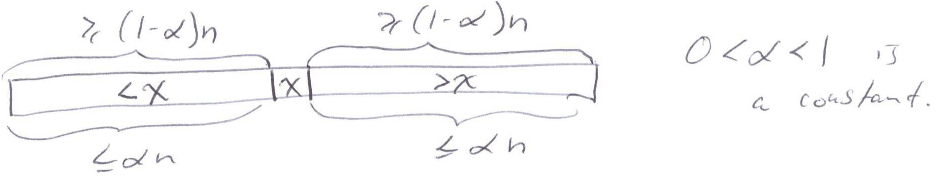
\includegraphics[scale=0.6]{selection}
  %\caption{Desirable properties of element x.}
  \label{fig:selection}
}

$x$ is somewhere around the middle of the array, and is preceded only
by elements smaller than $x$, and followed only by elements larger
than $x$.  We also know that there are $ \geq (1-\alpha)n $ and $ \leq
\alpha n $ elements both before and after $x$.

We can calculate this $x$ as follows:

\begin{enumerate}

\item Split $A$ into groups of 5.  There will be $\frac{n}{5}$ of
  these groups.
\item Compute the median $m_j$ of each group $M_j$ for $ 1 \leq j \leq
  \frac{n}{5} $.
\item Compute the median $x$ of $m_1,m_2,...,m_{n/5}$.

\end{enumerate}

It should be clear that step 1 takes constant time, step 2 takes
constant time for each group of constant size and $O(n)$ time total
for all $\frac{n}{5}$ groups, and step 3 takes $T(n/5)$ time.

\begin{claim}
This $x$ has the properties we needed above.
\end{claim}

\begin{proof}

We know that $\frac{1}{2}$ of $m_j$ are smaller than $x$, and since
there are $ \frac{n}{5} m_j$s, we know $\frac{n}{10}$ of $m_j$ are $
\leq x $.

So for each $m_j$ where $m_j \leq x$ 

\begin{itemize} 

\item there are 3 elements that are $ \leq m_j $
\item so 3 (or more) elements are $ \leq x $

\end{itemize}
%
\end{proof}
%
Now we must put $x$ into its position in the array using partitioning.
As a side note, partitioning is used in quicksort.

\begin{enumerate}

\item Find $x$, put it at the end
\item Partition elements around $x$
\item Put $x$ into its proper position

\end{enumerate}

We now have an $x$ that satisfies the properties we needed, and it is
properly located at position $q$ in $A$.  We are left with 3 cases:

\begin{enumerate}

\item If $i = q$: $x$ is the $i$-th element of $A$.
\item If $i < q$: recurse on the subarray which is $ < x $

\item If $i > q$: recurse on the subarray which is $ > x $, and $ i
  \leftarrow i - q $

\end{enumerate}

This last step gives a recurrence of $ T \left( \frac{7n}{10} \right)
$ in the worst case because at least $ \frac{3n}{10} $ elements in $A$
are smaller than $x$.

\section{Analysis}

We now have the following recurrence:
%
\begin{displaymath}
T(n) = T \left( \frac{n}{5} \right) +T \left( \frac{7n}{10} \right) + O(n)
\end{displaymath}

\begin{claim}
$ T(n) \leq cn $
\end{claim}

\begin{proof}
\begin{align*}
T(n)
&= dn + T \left( \frac{n}{5} \right) +T \left( \frac{7n}{10} \right) \\
&\leq dn + c \frac{n}{5} + c \frac{7n}{10} \\
&= dn + \frac{9}{10}cn \\
&= cn \left( \frac{d}{c} + \frac{9}{10} \right)
&\leq cn
\end{align*}

As long as

\begin{align*}
\frac{d}{c} + \frac{9}{10} &\leq 1 \\
\frac{d}{c} &\leq \frac{1}{10} \\
10 d &\leq c
\end{align*}
\end{proof}

\section{What is special about 5?}

First of all, we need an odd number for there to be a median.
Secondly, notice:
%
\begin{displaymath}
\frac{1}{5} + \frac{7}{10} = \frac{9}{10} < 1
\end{displaymath}

Dividing into groups of 3 doesn't work because:
%
\begin{displaymath}
T(n) = O(n) + T(n/3) + T(2n/3) = \Theta(nlogn)
\end{displaymath}

Dividing into groups of 7 actually does work because:
%
\begin{displaymath}
T(n) = O(n) + T(n/7) + T(5n/7) = \Theta(n)
\end{displaymath}
